\chapter{الگوریتم بهینه‌سازی}
در این فصل ابتدا سیستم مدل و چنل مدل را بیان میکنیم و سپس تکنیک ساده‌کردن مسئله به کمک متغیرهای واسط را شرح میدهیم. در ادامه، الگوریتم اصلی حل مسئله یعنی بهینه‌سازی دوره‌ای را مرور میکنیم و سپس دوگانه لاگرانژ و الگوریتم جستجوی ریشه دوبخشی را توضیح مختصری میدهیم و به کمک آنها، ضرایب آنتن را بهینه میکنیم. سپس ضرایب فاز را بکمک روش معروف گرادیان نزولی بهینه‌سازی کرده و در نهایت، 3 ناحیه اصلی بهینه‌سازی ضرایب فاز را شرح میدهیم. 
\newpage
%%%%%%%%%%%%%%%%%%%%%%%%%%%%%%%%%%%%%%%%%%%
\section{
	مدل سیستم و مدل کانال و مسئله بهینه‌سازی
}

\subsection{مدل سیستم}
طبق سناریویی که در فصل قبل شرح دادیم، سیگنال دریافتی در هر کاربر به شرح زیر می‌باشد:
\begin{equation}
	x = \sum_{k=1}^{K} w_k s_k, \label{eq:transmitted_signal}
\end{equation}
که دیتای کاربر \lr{k} ام توسط $s_k$ نمایش داده میشود. همچنین فرض میشود که این $s_k$ ها به ازای ($k = 1, \ldots, K$) متغیرهای رندوم و مستقل با میانگین صفر و واریانس 1 باشند.\\
از طرفی $w_k \in \mathbb{C}^{N_t \times 1}$ بردار ضرایب آنتن فرستنده هستند.\\
اکنون سیگنال دریافتی برای کاربر \lr{k} ام به شرح زیر قابل ساده‌سازی میباشد:
\begin{align*}
	y_k = &\underbrace{h_{d,k}^H x}_
	{\substack{\text{لینک مستقیم}}}
	\quad + \quad \\
	&\underbrace{h_{r_1,k}^H \Phi_1 G_1 x}_
	{\substack{\text{بازتاب مرتبه اول سطح هوشمند 1}}}
	\quad + \quad
	\underbrace{h_{r_2,k}^H \Phi_2 G_2 x}_
	{\substack{\text{بازتاب مرتبه اول سطح هوشمند 2}}}
	\quad + \quad \\ 
	&\underbrace{h_{r_1,k}^H \Phi_1 D \Phi_2 G_2 x}_
	{\substack{\text{بازتاب مرتبه دوم سطح هوشمند}}}
	\quad + \quad
	\underbrace{h_{r_2,k}^H \Phi_2 D^H \Phi_1 G_1 x}_
	{\substack{\text{بازتاب مرتبه دوم سطح هوشمند}}} \quad + \quad
	\underbrace{u_k}_
	{\substack{\text{نویز سفید گاوسی جمع‌شونده}}}
\end{align*}

بگونه‌ای که $u_k \sim \mathcal{CN}(0, \sigma_0^2)$ نشان‌دهنده نویز گاوسی در کاربر \lr{k} ام میباشد.
\newpage
اکنون به سراغ نوشتن نسبت سیگنال به نویز بعلاوه تداخل(\lr{SINR}) میرویم.\\
برای هر کاربر، نویز گاوسی بعلاوه سیگنال کاربران دیگر بعنوان سیگنال مزاحم تلقی شده و در مخرج کسر قرار میگیرند. پس \lr{SINR} کاربر \lr{k} به شکل زیر است:
\[
\gamma_k = \frac{{\left|\left(h_{d,k}^H + h_{r_1,k}^H \Phi_1 G_1 + h_{r_2,k}^H \Phi_2 G_2 + h_{r_1,k}^H \Phi_1 D \Phi_2 G_2 + h_{r_2,k}^H \Phi_2 D^H \Phi_1 G_1 \right)w_k\right|^2}}{{\sum_{i=1,i\neq k}^{K} \left|\left(h_{d,k}^H + h_{r_1,k}^H \Phi_1 G_1 + h_{r_2,k}^H \Phi_2 G_2 + h_{r_1,k}^H \Phi_1 D \Phi_2 G_2 + h_{r_2,k}^H \Phi_2 D^H \Phi_1 G_1 \right)w_i\right|^2 + \sigma^2_0}}
\]
همچنین شرط توان نیز برای مجموع کاربران به‌شکل زیر نوشته میشود:
\[
\sum_{k=1}^{K} ||w_k||^2 \leq P_T
\]
بگونه‌ای که:
$\mathbf{W} = [\mathbf{w}_1, \mathbf{w}_2, \ldots, \mathbf{w}_K] \in \mathbb{C}^{N_t \times K}$

\subsection{مدل کانال}
برای مدل کردن کانال، ابتدا از مدل‌های رندوم استفاده مینماییم اما در صورت جواب گرفتن از الگوریتم، آن‌را برای مدل‌های رایلی و رایسی نیز بهینه‌سازی میکنیم.

\subsection{مسئله بهینه‌سازی}
در این پروژه، هدف، بیشینه‌کردن مجموع نرخ دریافتی کاربران است که به آن \lr{WSR} گفته میشود. برای اینکار میبایست ضرایب آنتن و ضرایب فاز سطوح هوشمند را بصورت همزمان و توام بهینه‌سازی نماییم زیرا این دو دسته از متغیرها بر یکدیگر تاثیر میگذارند و نمیتوانند بصورت جداگانه بهینه‌سازی شوند. همچنین باید هر جوابی که برای ضرایب آنتن ارائه میشود، در شرط توان صدق نماید. پس مسئله را میتوان به شکل زیر فرموله کرد:
\begin{align*}
	(P1) \quad \max_{\mathbf{W}, \boldsymbol{\Phi_1}, \boldsymbol{\Phi_2}} \quad & f_1(\mathbf{W}, \boldsymbol{\Phi_1}, \boldsymbol{\Phi_2}) = \sum_{k=1}^{K} \omega_k \log_2(1 + \gamma_k) \\
	\text{به شرط} \quad & \theta_{m_k} \in \mathcal{F}, \quad \forall m_k = 1, \ldots, M_k, \tag{4-2} \\
	& \sum_{k=1}^{K} \| \mathbf{w}_k \|_2^2 \leq P_T,
\end{align*}

%%%%%%%%%%%%%%%%%%%%%%%%%%%%%%%%%%%%%%%%%%%
\section{الگوریتم بهینه‌سازی متناوب}
در این بخش، الگوریتم \lr{Alternating optimization} 
\cite{13}, \cite{14}
یا بهینه‌سازی پی‌در‌پی که به الگوریتم \lr{Coordinate Descent } یا مختصات نزولی نیز معروف میباشد را تعریف و نحوه بکارگیری آنرا شرح خواهیم داد.
\subsection{تعریف}
الگوریتم‌های هماهنگ نزولی مسائل بهینه‌سازی را با حداقل‌سازی تقریبی در امتداد جهت‌های مختصاتی یا ابرصفحه مختصاتی حل می‌کنند. این روش سال‌هاست که در برنامه‌های کاربردی مورد استفاده قرار می‌گیرد و محبوبیت آن‌ به دلیل مفید بودنش در تجزیه و تحلیل داده‌ها، یادگیری ماشین و دیگر زمینه‌های مورد علاقه فعلی، همچنان در حال رشد است.

\subsection{استفاده}
در مسئله بهینه‌سازی فعلی، 2 دسته اصلی پارامتر داریم که باید بهینه‌سازی شوند. دسته اول مربوط به ضرایب آنتن میباشد که یک بردار با طول مشخص است. دسته دوم مربوط به ضرایب سطوح هوشمند است که خود به 2 دسته تقسیم میشوند زیرا 2 سطح هوشمند مستقل از هم داریم. البته لازم به ذکر است که در ادامه و با بوجود آمدن متغیرهای کمکی در طول مسئله، این دسته از متغیرها نیز به پارامترهای بهینه‌سازی اضافه میشوند که طول عمر آنها بصورت محلی تعریف میشود و جزو پارامترهای اصلی مسئله نیستند.

پس به طول کلی یک حلقه داریم که ابتدا ضرایب اولیه‌ای را برای فاز سطوح هوشمند در نظر گرفته و ضرایب آنتن‌ را بهینه‌سازی مینماییم. سپس ضرایب آنتن را ثابت فرض کرده و ضرایب سطوح هوشمند را بهینه‌سازی مینماییم.
\begin{figure}[!h]
	\centering
	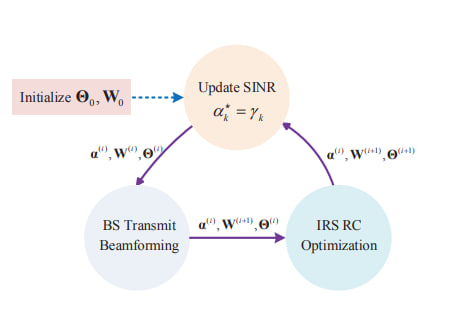
\includegraphics[scale=0.65]{AO}
	
	\caption[شیوه استفاده الگوریتم مختصات نزولی در پروژه]{
		شیوه استفاده الگوریتم مختصات نزولی در پروژه
	}
	%	\label{fig:fig-2_03}
\end{figure}
%%%%%%%%%%%%%%%%%%%%%%%%%%%%%%%%%%%%%%%%%%%
\section{تبدیل دوگان لاگرانژی}
یکی از مشکلاتی که در این مسئله بهینه‌سازی و همه مسائل مرتبط با بهینه‌سازی حداکثر نرخ قابل‌دسترسی با آن روبرو هستیم، وجود تابع لاگاریتم میباشد. اگر فقط یک عدد تابع لگاریتم وجود داشت، به علت اینکه لگاریتم تابعی اکیدا یکنوا (اکیدا صعودی) است، میتوانستیم آن را حذف کرده و فقط تابع جلوی لگاریتم را بهینه‌سازی نماییم اما در اینجا با جمع چند لگاریتم روبرو هستیم. شاید یک راه حل احتمالی این باشد که از قانون تبدیل جمع به ضرب در لگاریتم استفاده شود اما این خود باعث افزایش پیچیدگی مسئله میشود. 
\subsection{تعریف}
اکنون که مشکل را درک کردیم، به سراغ معروف‌ترین راه‌حل آن میرویم. یکی از تبدیل‌هایی که میتوان جهت حذف لگاریتم در چنین مسائلی استفاده نمود، تبدیل دوگانی لاگرانژ لگاریتمی میباشد. 
این تبدیل توسط دو عضو جامعه علمی برق در سال 2018 در بخش دوم مقاله‌ای جهت استفاده برای حل مسائل مخابرات ارائه گردید.

تکنیک به گونه‌ای میباشد که با اضافه کردن پارامترهایی اختیاری به نام آلفا به مسئله، باعث جابجایی تابع جلوی لگاریتم به بیرون آن میشود و عملا با حذف لگاریتم، باعث ساده‌شدن مسئله بهینه‌سازی میشود. در ادامه از این تکنیک پرکاربرد استفاده خواهیم‌نمود.
\subsection{ساده‌سازی مسئله}
این تکنیک در مسئله ما به‌صورت زیر قابل استفاده میباشد:
\[
f_{1a}(\mathbf{W}, \boldsymbol{\Theta}, \boldsymbol{\alpha}) = \sum_{k=1}^{K} \omega_k \log_2(1 + \alpha_k) - \sum_{k=1}^{K} \omega_k \alpha_k + \sum_{k=1}^{K} \frac{\omega_k (1 + \alpha_k) \gamma_k}{1 + \gamma_k}
\]
همانطور که مشاهده میشود، مسئله 4-2 قابل تبدیل به مسئله بالا میباشد که پارامتر اختیاری آلفا به تعداد کاربران به مسئله اضافه شده‌است.

همچنین گاما همان نسبت سیگنال به نویز معروف میباشد.
اکنون شاید این سوال پیش بیاید که آیا با اضافه‌شدن یک دسته پارامتر جدید، چگونه باعث ساده‌تر شدن مسئله میشویم؟

جواب این سوال وقتی مشخص میشود که به کمک الگوریتم مختصات نزولی شروع به بهینه‌سازی این دو دسته پارامتر نماییم:

1- دسته اول همان پارامترهای آنتن و سطوح هوشمند

2- دسته دوم پارامترهای اختیاری اضافه‌شده به مسئله

برای اینکار، ابتدا پارامترهای دسته اول را ثابت فرض میکنیم و نسبت به پارامترهای دسته دوم مشتق میگیریم.
نکته قابل‌توجه اینکه این مشتق‌گیری به سادگی قابل انجام است و با صفر قرار دادن آن، مقدار بهینه آلفا به شکل زیر یافت میشود:

 \[\alpha_k^\circ = \gamma_k\]

 اکنون با ثابت فرض کردن آلفا، مسئله به شکل زیر تبدیل میشود و به سراغ بهینه‌سازی پارامترهای دسته اول میرویم :
 
 \[
 (P1'') \quad \max \mathbf{W}, \boldsymbol{\Theta} \quad \sum_{k=1}^{K} \frac{\alpha_k^\sim \gamma_k}{1 + \gamma_k}
 \]
 
 بگونه‌ای که $\alpha_k^\sim = \omega_k(1 + \alpha_k)$ میباشد.
 
 اکنون به مجموع چند عبارت کسری رسیدیم که در ادامه با استفاده از تکنیک برنامه‌ریزی چند کسری به حل این مسئله میپردازیم.
%%%%%%%%%%%%%%%%%%%%%%%%%%%%%%%%%%%%%%%%%%%
\section{برنامه‌ریزی چند کسری}
\cite{12}
اکنون با چند کسر مواجه هستیم که مشتق‌گرفتن از آنها و حل معادله حاصله به راحتی امکان‌پذیر نیست. پس لازم است از تبدیل دیگری به‌نام برنامه‌ریزی چند کسری استفاده نماییم تا این مسئله به فرم خطی تبدیل شود بگونه‌ای که مسئله حاصله، معادل مسئله اصلی باشد یعنی نقاط بهینه یکسانی داشته باشند. 

\subsection{تعریف}
این تبدیل در بخش اول مقاله‌ای که در بخش قبل به آن اشاره شد معرفی شده‌است. همانند تبدیل معرفی شده در بخش قبل و سایر تبدیل‌ها، یک دسته پارامتر اختیاری بنام بتا به مسئله اضافه میشوند که البته باعث ساده‌شدن مسئله بهینه‌سازی میشود.\\
در ادامه به نحوه استفاده از این تکنیک در مسئله میپردازیم.
\subsection{ساده‌سازی مسئله}
ابتدا برای ساده‌سازی نوشتار، یک پارامتر جدید مربوط به کانال‌ها تعریف میکنیم:
\[\mathbf{h}_k = \mathbf{h}_d,k + \mathbf{GH}\boldsymbol{\Theta}\mathbf{h}_r,k\]
پس نسبت سیگنال به نویز به شکل زیر تغییر میکند:
\[
\gamma_k = \frac{{\lVert \mathbf{h}_k \mathbf{w}_k \rVert^2}}{{\sum_{i=1,i\neq k}^{K} \lVert \mathbf{h}_k \mathbf{w}_i \rVert^2 + \sigma_0^2}}
\]
اکنون با استفاده از تبدیل کسری و اضافه شدن پارامتر بتا، مسئله بهینه‌سازی به شکل زیر تغییر میکند و به فرم خطی نوشته می‌شود:
\[
f2a(\mathbf{W}, \boldsymbol{\beta}) = \sum_{k=1}^{K} 2 \sqrt{\alpha_k^\sim} \Re \left\{ \beta_k^* \mathbf{h}_k^H \mathbf{w}_k \right\} - \sum_{k=1}^{K} \lvert \beta_k \rvert^2 \sum_{i=1}^{K} \lVert \mathbf{h}_k \mathbf{w}_i \rVert^2 + \sigma_0^2.
\]
بگونه‌ای که دامنه بتا برابر اعداد مختلط باشد.
%%%%%%%%%%%%%%%%%%%%%%%%%%%%%%%%%%%%%%%%%%%
\section{بهینه‌سازی ضرایب آنتن}
اکنون دوباره با بکارگیری الگوریتم مختصات نزولی یا \lr{Coordinate Descent} میتوان پارامتر های بتا و سایر پارامترها را در داخل یک حلقه، بهینه‌سازی کرد.\\
برای اینکار میبایست ابتدا نسبت به بتا مشتق گرفته و مقدار بهیه آن را بدست آوریم. این کار به سادگی قابل انجام است. 

\subsection{مقدار بتا بهینه}
مقدار بهینه بتا در زیر آورده شده‌است:
\[
\beta_k^* = \sqrt{\alpha_k^\sim} \frac{{\mathbf{h}_k^H \mathbf{w}_k}}{{\sum_{i=1}^{K} \lVert \mathbf{h}_k \mathbf{w}_i \rVert^2 + \sigma_0^2}}.
\]
\subsection{مقدار بهینه بردار آنتن}
اکنون نوبت به بهینه‌سازی اولین دسته پارامتر اصلی مسئله یعنی ضرایب فعال آنتن رسیده است. همانند سایر پارامترها برای بدست آوردن مقدار بهینه آن، نسبت به \lr{W} مشتق گرفته و برابر صفر قرار میدهیم. نتیجه در رابطه زیر قابل مشاهده‌است:
\[\mathbf{w}_k^* = \sqrt{\alpha_k^\sim} \beta_k \left( \lambda_0 \mathbf{I}_M + \sum_{i=1}^{K} \lvert \beta_i \rvert^2 \mathbf{h}_i \mathbf{h}_i^H \right)^{-1} \mathbf{h}_k,
\]
البته لازم به ذکر است چون بر روی این دسته پارامتر، شرط توان نیاز است رعایت شود باید یک پارامتر کمکی به نام لامبدا به مسئله اضافه کنیم که با تغییر آن، شرط توان را برقرار سازیم.
مقدار لامبدا به صورت بهینه توسط حل نامعادله زیر بدست می‌آید:
\[
\lambda_0^* = \min \left( \lambda_0 \geq 0 : \sum_{k=1}^{K} \lVert \mathbf{w}_k \rVert^2 \leq PT \right).
\]
روش حل این نامعادله را توسط سریع‌ترین روش یعنی جستجوی دوبخشی در زیر توضیح خواهیم داد. 
\subsection{روش جستجوی دوبخشی}
یکی از ساده‌ترین و در عین حال بهینه‌ترین روش‌های جستجوی ریشه تابع در یک بازه، روش جستجوی دو بخشی یا \lr{Bisection Search}
میباشد. این روش میتواند به طور همزمان فقط یک ریشه را در یک بازه مشخص پیدا کند. برای اطمینان از وجود ریشه در یک بازه، طبق قضیه مقدار میانی، مقدار تابع باید در ابتدا و انتهای بازه مختلف‌العلامه باشند. این روش ابتدا وسط بازه را به عنوان نقطه سوم در نظر گرفته و مقدار آن را در تابع حساب میکند. سپس بازه جستجوی جدید بین نقطه سوم و نقطه‌ایست که علامت متفاوتی با نقطه سوم دارد. به همین روش بازه جستجو را کوچک کرده و در نهایت با یک شرط پایان مثلا تعیین شرط میزان خطا بر روی ریشه، الگوریتم متوقف میشود.

\subsection{حد بالای لامبدا}
یکی از مسائلی که در روش دو بخشی باید پیش از اجرای الگوریتم تعیین کنیم، نقطه شروع و پایان الگوریتم میباشد. نقطه شروع برای این مسئله همیشه از صفر میباشد اما حد بالای آن چگونه یافت میشود؟

- یک روش آنست که مقداری بسیار بزرگ برای آن قرار دهیم که اتفاقا در اکثر سناریوها روشی قابل انجام است اما به علت محاسبات سنگین‌تر با اعداد بزرگتر، باعث کند شدن الگوریتم و به علت بزرگ‌ بودن بازه جستجو، دیرتر به ریشه تابع همگرا میشود.

- اما در روش دوم، طبق مقاله [] میتوان از ضابطه زیر جهت حد بالای پارامتر لامبدا استفاده نمود:
\[
	g(\lambda) \leq \sum_{k=1}^{K}\left|\alpha_{k}\right|^{2}\left|q_{k}\right|^{2} \sum_{i=1}^{N} \frac{\left[\mathbf{Z}_{k}\right]_{i, i}}{\lambda_{\max }^{2}} \triangleq P_{\max }, \\
	\Rightarrow \lambda_{\max }=\sqrt{\frac{\sum_{k=1}^{K}\left|\alpha_{k}\right|^{2}\left|q_{k}\right|^{2} \sum_{i=1}^{N}\left[\mathbf{Z}_{k}\right]_{i, i}}{P_{\max }} .}
\]
از طریق روابط زیر نیز قابل اثبات است:
\[
	g(\lambda)  =\sum_{k=1}^{K}\left\|\mathbf{w}_{k}\right\|_{2}^{2}=
\]
\[
\sum_{k=1}^{K} \operatorname{Tr}\left(\mathbf{F}_{1}\left(\boldsymbol{\Sigma}_{1}+\lambda \mathbf{I}\right)^{-1} \mathbf{F}_{1}^{H} \alpha_{k} q_{k} \overline{\mathbf{h}}_{k} u_{k} u_{k}^{H} \overline{\mathbf{h}}_{k}^{H} q_{k} \alpha_{k} \mathbf{F}_{1}\left(\boldsymbol{\Sigma}_{1}+\lambda \mathbf{I}\right)^{-1} \mathbf{F}_{1}^{H}\right)=
\]
\[
	 \sum_{k=1}^{K}\left|\alpha_{k}\right|^{2}\left|q_{k}\right|^{2} \operatorname{Tr}\left(\left(\boldsymbol{\Sigma}_{1}+\lambda \mathbf{I}\right)^{-2} \mathbf{F}_{1}^{H} \overline{\mathbf{h}}_{k} u_{k} u_{k}^{H} \overline{\mathbf{h}}_{k}^{H} \mathbf{F}_{1}\right) \\
	 =\sum_{k=1}^{K}\left|\alpha_{k}\right|^{2}\left|q_{k}\right|^{2} \sum_{i=1}^{N} \frac{\left[\mathbf{Z}_{k}\right]_{i, i}}{\left(\varepsilon_{i}+\lambda\right)^{2}},
\]
%%%%%%%%%%%%%%%%%%%%%%%%%%%%%%%%%%%%%%%%%%%
\section{بهینه‌سازی ضرایب فاز سطوح هوشمند}
اکنون سراغ بهینه‌سازی دسته دوم از پارامترهای اصلی مسئله میرویم. دوباره برای تبدیل کسر به عبارتی خطی، نیاز است از برنامه‌ریزی چند کسری استفاده نماییم که در زیر قابل مشاهده است(اینبار با پارامتر اپسیلون این کار را انجام میدهیم):
\[
	f_{3 a}(\boldsymbol{\theta}, \boldsymbol{\varepsilon})=  \sum_{k=1}^{K} 2 \sqrt{\tilde{\alpha}_{k}} \operatorname{Re}\left\{\varepsilon_{k}^{*} \boldsymbol{\theta}^{\mathrm{H}} \mathbf{a}_{k, k}+\varepsilon_{k}^{*} b_{k, k}\right\} \\
	 -\sum_{k=1}^{K}\left|\varepsilon_{k}\right|^{2}\left(\sum_{i=1}^{K}\left|b_{i, k}+\boldsymbol{\theta}^{\mathrm{H}} \mathbf{a}_{i, k}\right|^{2}+\sigma_{0}^{2}\right)
\]

\subsection{مقدار اپسیلون بهینه}
همانند بخش قبل که مقدار بهینه بتا را بدست آوردیم، اکنون به سراغ محاسبه مقدار بهینه اپسیلون میرویم:\
\[
\varepsilon_{k}^{\circ}=\frac{\sqrt{\tilde{\alpha}_{k}}\left(b_{k, k}+\boldsymbol{\theta}^{\mathrm{H}} \mathbf{a}_{k, k}\right)}{\sum_{i=1}^{K}\left|b_{i, k}+\boldsymbol{\theta}^{\mathrm{H}} \mathbf{a}_{i, k}\right|^{2}+\sigma_{0}^{2}} .
\]
\newpage
\subsection{روش گرادیان نزولی}
\cite{15}
این الگوریتم بهینه‌سازی، در عین مفهوم بسیار ساده‌ای که دارد، یک روش بسیار پرکاربرد و در صورت انتخاب کردن طول گام مناسب، بسیار سریع است.\\
برای پیدا کردن کمینه محلی، کافیست تابع مشتق‌پذیر باشد تا از آن مشتق گرفته و در جهت خلاف آن حرکت نماییم. 
برای پیدا کردن بیشینه، کافیست در جهت مشتق حرکت نماییم.
لازم به ذکر است که همه الگوریتم‌ها نقاط بهینه‌ محلی میدهند و اگر تابع محدب باشد، آن نقطه بهینه محلی، بهینه سراسری نیز می‌باشد.\\
در این روش نیاز به انتخاب طول گام داریم که سرعت همگرایی را مشخص می کند. اگر طول گام خیلی کوچک باشد، ممکن است دیر همگرا شود. اگر طول گام خیلی بزرگ انتخاب شود، ممکن است در بهینه محلی گیر نکند. پس باید مقداری مناسب برای آن قرار دهیم که روش‌های زیادی نیز برای انتخاب طول گام به شکلی تطبیق‌پذیر یا \lr{adaptive} نوشته شده‌است.

\newpage
\subsection{ضرایب بهینه سطوح هوشمند یک و دو}
برای محاسبه مقدار بهینه تتا میتوان دوباره مشتق گرفت ولی این روش سرعت کمی دارد و بهتر است از روش گرادیان نزولی برای یک بردار استفاده نماییم.

ابتدا چند تعریف ساده ارائه میدهیم:
\[
	\left|b_{i, k}+\boldsymbol{\theta}^{\mathrm{H}} \mathbf{a}_{i, k}\right|^{2}  =\left(b_{i, k}+\boldsymbol{\theta}^{\mathrm{H}} \mathbf{a}_{i, k}\right)\left(b_{i, k}^{*}+\mathbf{a}_{i, k}^{\mathrm{H}} \boldsymbol{\theta}\right) \\
	 =\boldsymbol{\theta}^{\mathrm{H}} \mathbf{a}_{i, k} \mathbf{a}_{i, k}^{\mathrm{H}} \boldsymbol{\theta}+2 \operatorname{Re}\left\{b_{i, k}^{*} \boldsymbol{\theta}^{\mathrm{H}} \mathbf{a}_{i, k}\right\}+\left|b_{i, k}\right|^{2}
\]
\[	f_{4}(\boldsymbol{\theta})  =f_{3 a}\left(\boldsymbol{\theta}, \boldsymbol{\varepsilon}^{\circ}\right) \\
	 =-\boldsymbol{\theta}^{\mathrm{H}} \boldsymbol{R} \boldsymbol{\theta}+2 \operatorname{Re}\left\{\boldsymbol{\theta}^{\mathrm{H}} \boldsymbol{e}\right\}+C,
\]
\[	\boldsymbol{R}  =\sum_{k=1}^{K}\left|\varepsilon_{k}\right|^{2} \sum_{i=1}^{K} \mathbf{a}_{i, k} \mathbf{a}_{i, k}^{\mathrm{H}},
\]
\[
	\boldsymbol{e}  =\sum_{k=1}^{K}\left(\sqrt{\tilde{\alpha}_{k}} \varepsilon_{k}^{*} \mathbf{a}_{k, k}-\left|\varepsilon_{k}\right|^{2} \sum_{i=1}^{K} b_{i, k}^{*} \mathbf{a}_{i, k}\right),
\]
\[
	C  =\sum_{k=1}^{K}\left(2 \sqrt{\tilde{\alpha}_{k}} \operatorname{Re}\left\{\varepsilon_{k}^{*} b_{k, k}\right\}-\left|\varepsilon_{k}\right|^{2}\left(\sigma_{0}^{2}+\sum_{i=1}^{K}\left|b_{i, k}\right|^{2}\right)\right)
\]

ابتدا به کمک گرادیان نزولی و مپ کردن جواب بر روی دایره واحد، مقدار گرادیان را از طریق رابطه زیر محاسبه میکنیم:
\[
\nabla_{\Theta} f_{4}=2 \operatorname{Re}\left\{(\mathbf{R \theta}-\mathbf{e})^{*} \odot(-j \mathbf{\theta})\right\},
\]
اکنون به کمک مفهوم روش \lr{iterative} گرادیان نزولی، مقدار جدید ضرایب فاز سطح هوشمند شماره 1 را از ترکیب مقدار قبلی بهمراه ضریبی از تغییرات (گرادیان) توسط رابطه زیر بدست می‌آوریم:
\[
\boldsymbol{\Theta}^{(t+1)}=\boldsymbol{\Theta}^{(t)}-\gamma^{(t)} \nabla_{\boldsymbol{\Theta}} f\left(\mathbf{X}^{(t)}\right),
\]
محاسبه ضرایب سطح هوشمند شماره 2 نیز به روش مشابه قابل انجام است.
\newpage
\subsection{سه ناحیه اصلی بهینه‌سازی ضرایب فاز}
برای بهینه‌سازی ضرایب فاز، 3 ناحیه اصلی وجود دارد که جواب نهایی را میتوان به آن ناحیه مپ کرد.

- ناحیه اول، ناحیه درون دایره واحد است که اکثر الگوریتم‌ها بصورت پیش‌فرض جواب را در این ناحیه میدهند. این ناحیه الزاما جواب بهینه سراسری نمیدهد زیرا همراه با کاهش توان همراه است (اندازه بردار داخل دایره واحد کمتر از 1 میباشد). 

- ناحیه دوم، ناحیه روی دایره یکه است. احتمال وجود بهینه‌ سراسری در این ناحیه بالا است. جواب های درون دایره واحد که از الگوریتم‌های مرحله قبل بدست می‌آید، به این ناحیه مپ میشوند یعنی اندازه بردار آنها برابر واحد میشود یا به عبارتی آن عدد مختلط را بر اندازه‌اش تقسیم میکنند.

- ناحیه سوم که ناحیه ایست که عملا کاربرد واقعی دارد، ناحیه کوانتیزه‌شده روی دایره یکه است. به عبارتی این ناحیه زیرمجموعه ناحیه قبل است و فقط شامل نقاط محدودی از آن میشود.  مثلا می‌توان کوانتیزیشن 9 بیتی انجام داد که حدودا خطای یک درجه می‌دهد.

این مسئله بر روی ناحیه دوم حل شده است که به راحتی موقع پیاده‌سازی میتواند به نزدیک‌ترین نقطه در ناحیه سوم مپ شود.
%%%%%%%%%%%%%%%%%%%%%%%%%%%%%%%%%%%%%%%%%%%
\newpage
‌